\subsection{Herstellung von Optischen Wellenleitern}
\label{subsec:pofherstellungsverfahren}

\subsubsection{Herstellung einer SI-POF mittels Extrusion}

Für die Herstellung eines polymeren Wellenleiters mit Stufenindexprofil eignet
sich die kontinuirliche Extrusion (siehe \autoref{fig:pofsispinn}). Dabei werden
die Monomere samt Radikalstarter und Additiven in ein geheiztes
Polymerisationsgefäß (\textit{heating unit}) gegeben. Nachdem der Polymeranteil
in der Reaktionskammer hoch genug ist, werden diese in den Extruder gepumpt. Das
Polymer wird von dem Extruder in eine Spinndüse gedrückt. In der Spinndüse wird
der Kern des POFs geformt und mit einem Mantel aus dem Extruder mit dem
Mantelmaterial (\textit{cladding material}) versehen. Der Faden wird dann in
einer \textit{blow box} gekühlt, gedehnt (\textit{stretching}) und aufgerollt
(\textit{take-up}). Vorteilhaft bei diesem Verfahren ist die Eignung zur
Massenproduktion und die Reinheit des Kerns, da keine vorgefertigtes Granulat
verwendet wird. Ein Nachteil dagegen sind die hohen Kosten.

\begin{figure}[h]
    \begin{center}
        \begin{minipage}[t]{\textwidth}
            \begin{center}
                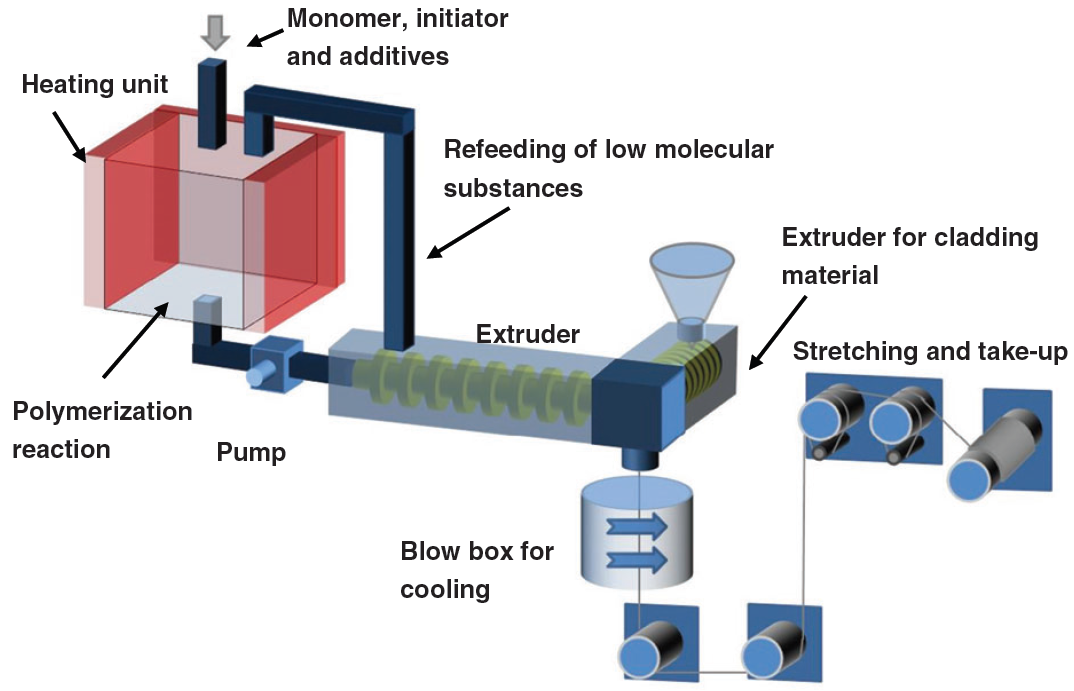
\includegraphics[height=0.25\textheight]{Bilder/Optische_Wellenleiter_Die_Polymer_Optische_Faser/Herstellung/pofsispinn.png}
                \caption[kontinuirliche Extrusion einer SI-POF \newline \url{http://www.researchgate.net/publication/265646639_An_overview_on_fabrication_methods_for_polymer_optical_fibers} S. 5 (zuletzt aufgerufen am 28.09.2015)]{kontinuirliche Extrusion einer SI-POF}
                \label{fig:pofsispinn}
            \end{center}
        \end{minipage}
    \end{center}
\end{figure}

Dieses Verfahren eignet sich ebenfalls für die Herstellung von POFs mit
\textit{Multi Step Index}. Dabei kommen jedoch mehrere Extruder zum Einsatz
(siehe \autoref{fig:pofmsispinn}), die nacheinander eine Schicht auf den Kern
auftragen und so mehrere übereinanderliegende Mäntel entstehen lassen.
\cite{pofspinn}

\begin{figure}[h]
    \begin{center}
        \begin{minipage}[t]{\textwidth}
            \begin{center}
                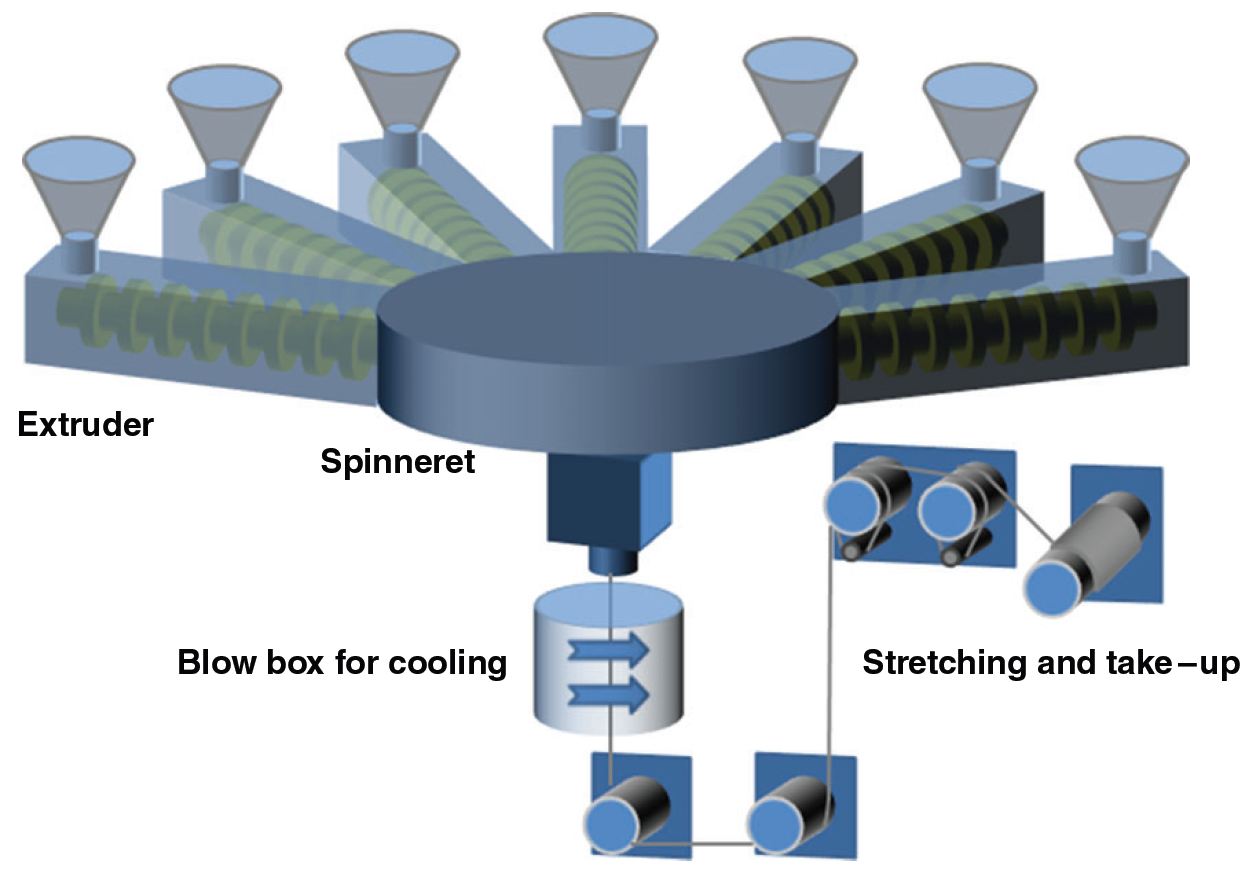
\includegraphics[height=0.25\textheight]{Bilder/Optische_Wellenleiter_Die_Polymer_Optische_Faser/Herstellung/pofmsispinn.png}
                \caption[kontinuirliche Extrusion einer SI-POF \newline \url{http://www.researchgate.net/publication/265646639_An_overview_on_fabrication_methods_for_polymer_optical_fibers} S. 5 (zuletzt aufgerufen am 28.09.2015)]{kontinuirliche Extrusion einer SI-POF}
                \label{fig:pofmsispinn}
            \end{center}
        \end{minipage}
    \end{center}
\end{figure}

\subsubsection{Herstellung einer GI-POF mittels eines modifiziertem Schmelzspinnprozesses}

Ein weiteres Herstellungsverfahren besteht in einem modifizierten
Schmelzspinnprozess der RWTH Aachen. Dieses Verfahren eignet sich für die
Herstellung von POFs mit einem Gradientenindexprofil. \autoref{fig:pofgispinn}
zeigt die nötige Produktionsanlage bestehend aus einem Einfülltrichter
(\textit{hopper}) für das granulierte Kernmaterial, einem Extruder, welcher das
Granulat erhitzt und in die Spinndüse (\textit{spinning nozzle}) drückt. Die
Spinndüse wandelt die erhitzte Kernmaterialmasse zu einem Faden um. Dieser wird
durch das Wasserbad (\textit{water quench}) gezogen. Dabei ist der
Abkühlungsvorgang für Gradientenindexprofil verantwortlich. Die Kühlungsraten
nehmen von außen nach innen ab und beinträchtigen damit die Dichte
beziehungsweise den Brechzahlenverlauf. In der letzten Einheit wird der
Polymerfaden gedehnt und aufgewickelt Die Vorteile dieses Verfahrens liegt zu
einem in der ununterbrochenen Produktion des Wellenleiters und der damit
verbundenen Wirtschaftlichkeit, da keine Unterbrechungen nötig sind, und zum
anderen in der Möglichkeit die Brechzahlen durch Variierung der Verweilzeit des
Fadens im Wasser und der Wassertemperatur zu beeinflussen.  \cite{pofspinn}

\begin{figure}[h]
    \begin{center}
        \begin{minipage}[t]{\textwidth}
            \begin{center}
                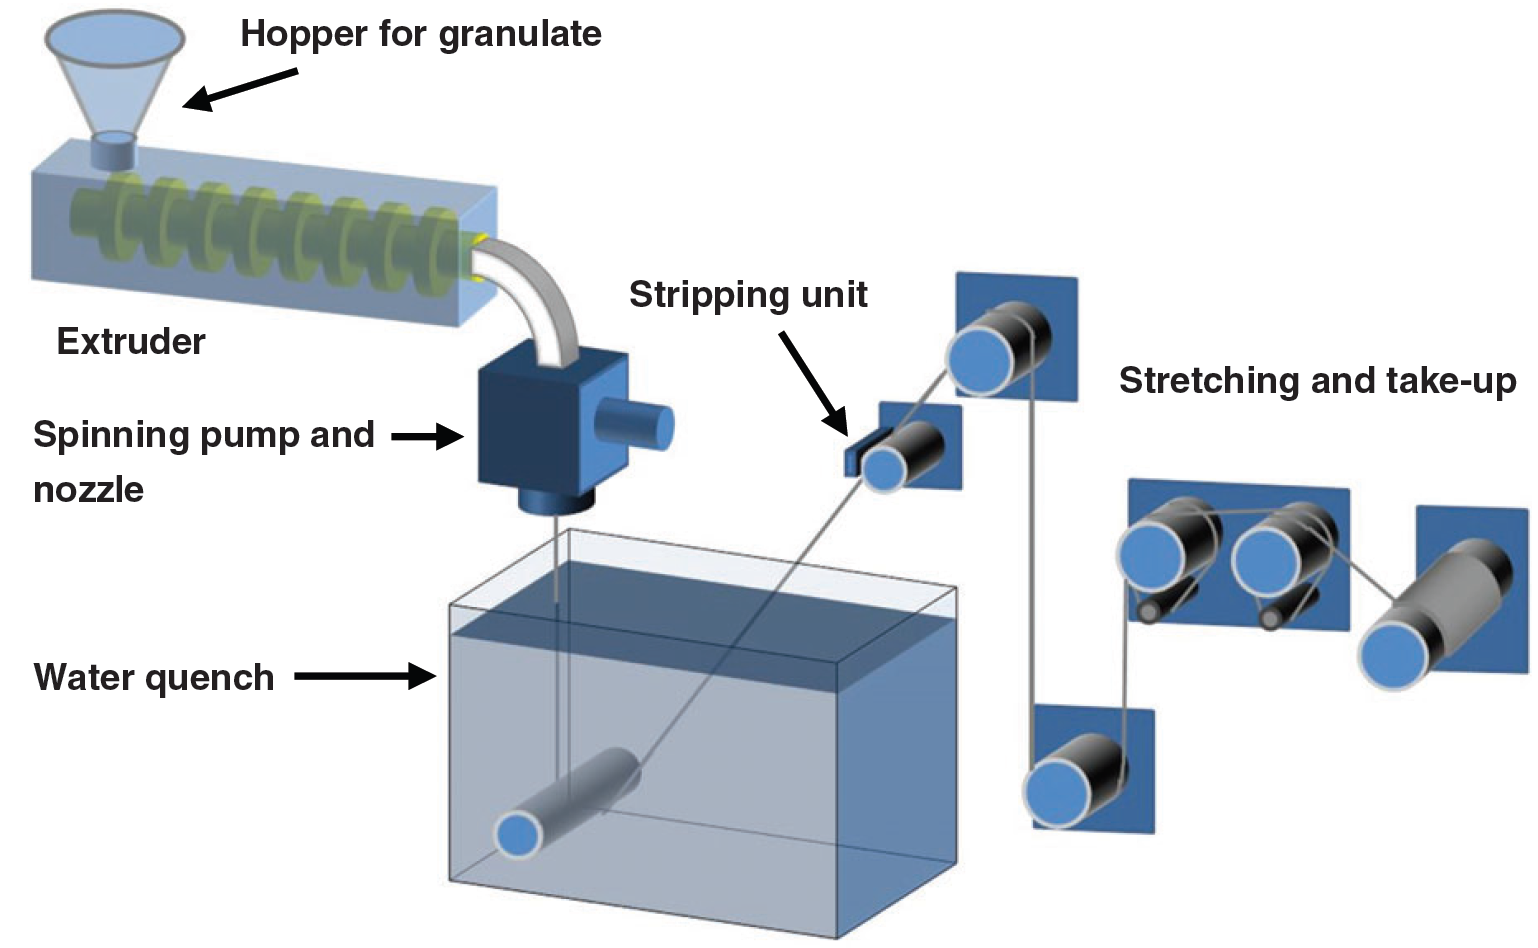
\includegraphics[height=0.25\textheight]{Bilder/Optische_Wellenleiter_Die_Polymer_Optische_Faser/Herstellung/pofgispinn.png}
                \caption[Schmelzspinnprozess zur Herstellung einer GI-POF \newline \url{http://www.researchgate.net/publication/265646639_An_overview_on_fabrication_methods_for_polymer_optical_fibers} S. 9 (zuletzt aufgerufen am 28.09.2015)]{Schmelzspinnprozess zur Herstellung einer GI-POF}
                \label{fig:pofgispinn}
            \end{center}
        \end{minipage}
    \end{center}
\end{figure}
